% Three-minute lightning talk on rdfc2im, BH26JP closing session.
% Build with `make` (XeLaTeX, run twice for the page-anchored overlays).
\documentclass[aspectratio=169,11pt]{beamer}

\usepackage{fontspec}
\setsansfont{Lato}[BoldFont={Lato Black}]
\newfontfamily\sealfont{Noto Serif CJK JP}[BoldFont={* Bold}]
\usepackage{tikz}
\usetikzlibrary{calc}
\graphicspath{{./}{../paper/}{logos/}}

% Colours from the report's Figure 1.
\definecolor{shared}{HTML}{3B5B86}
\definecolor{mine}{HTML}{3D7A45}
\definecolor{custom}{HTML}{B5561C}
\definecolor{ink}{HTML}{222222}
\definecolor{muted}{HTML}{555555}
\definecolor{vermilion}{HTML}{E34234}

\setbeamertemplate{navigation symbols}{}
\setbeamercolor{background canvas}{bg=white}
\setbeamercolor{normal text}{fg=ink}
\setbeamersize{text margin left=6mm, text margin right=6mm}

\newcommand{\headline}[1]{{\fontsize{16}{19}\selectfont\bfseries\color{shared}#1\par}}
\newcommand{\sub}[1]{{\fontsize{10.5}{13}\selectfont #1\par}}
\newcommand{\bignum}[2]{%
  \noindent\parbox[c]{28mm}{\raggedleft\fontsize{20}{21}\selectfont\bfseries\color{shared}#1}%
  \hspace{2.5mm}%
  \parbox[c]{\dimexpr\linewidth-30.5mm}{\raggedright\fontsize{9}{10.5}\selectfont #2}\par
  \vspace{3.2mm}}

\begin{document}

% ---------------------------------------------------------------- 1. The idea
\begin{frame}[t]
  \vspace*{-3mm}
  \headline{RDF Portal + rdf-config are enough to rebuild an InterMine}
  \vspace{1mm}
  \sub{The mapping is data, not code.}
  \vspace{2.5mm}
  \centering
  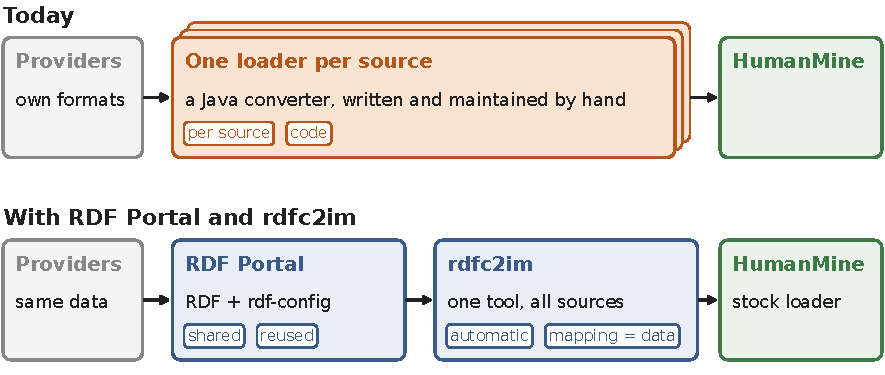
\includegraphics[width=0.92\paperwidth]{ecosystem.pdf}

  \begin{tikzpicture}[remember picture, overlay]
    \node[anchor=south, fill=shared!10, minimum width=\paperwidth, inner sep=1.4mm,
          text width=\paperwidth-12mm, align=left]
      at (current page.south)
      {\fontsize{6.5}{8}\selectfont
       \textbf{Building InterMine databases from RDF Portal}\enspace\textbullet\enspace
       Russell Y.\ Neches (Kyoto Univ.), Shuichi Kawashima, Toshiaki Katayama \mbox{(NIG / DBCLS)},
       Gos Micklem \mbox{(Univ.\ of Cambridge; NIG / DBCLS)}\enspace\textbullet\enspace DBCLS BioHackathon 2026};
  \end{tikzpicture}
\end{frame}

% ------------------------------------------------- 2 and 3. It works, then the seal
\begin{frame}[t]
  \vspace*{-3mm}
  \headline{It works: a HumanMine built from RDF Portal}
  \vspace{3mm}
  \begin{columns}[T, onlytextwidth]
    \begin{column}{0.38\textwidth}
      \bignum{9}{sources, 8 of them via RDF Portal}
      \bignum{113}{panel genes: food and drug metabolism}
      \bignum{193,288}{genes from NCBI Gene, in full}
      \bignum{53,105}{ClinVar alleles for the panel}
      \vspace{1mm}
      {\fontsize{10}{12}\selectfont\color{mine}\bfseries search \textbullet\ templates
       \textbullet\ list analysis\par}
    \end{column}
    \begin{column}{0.59\textwidth}
      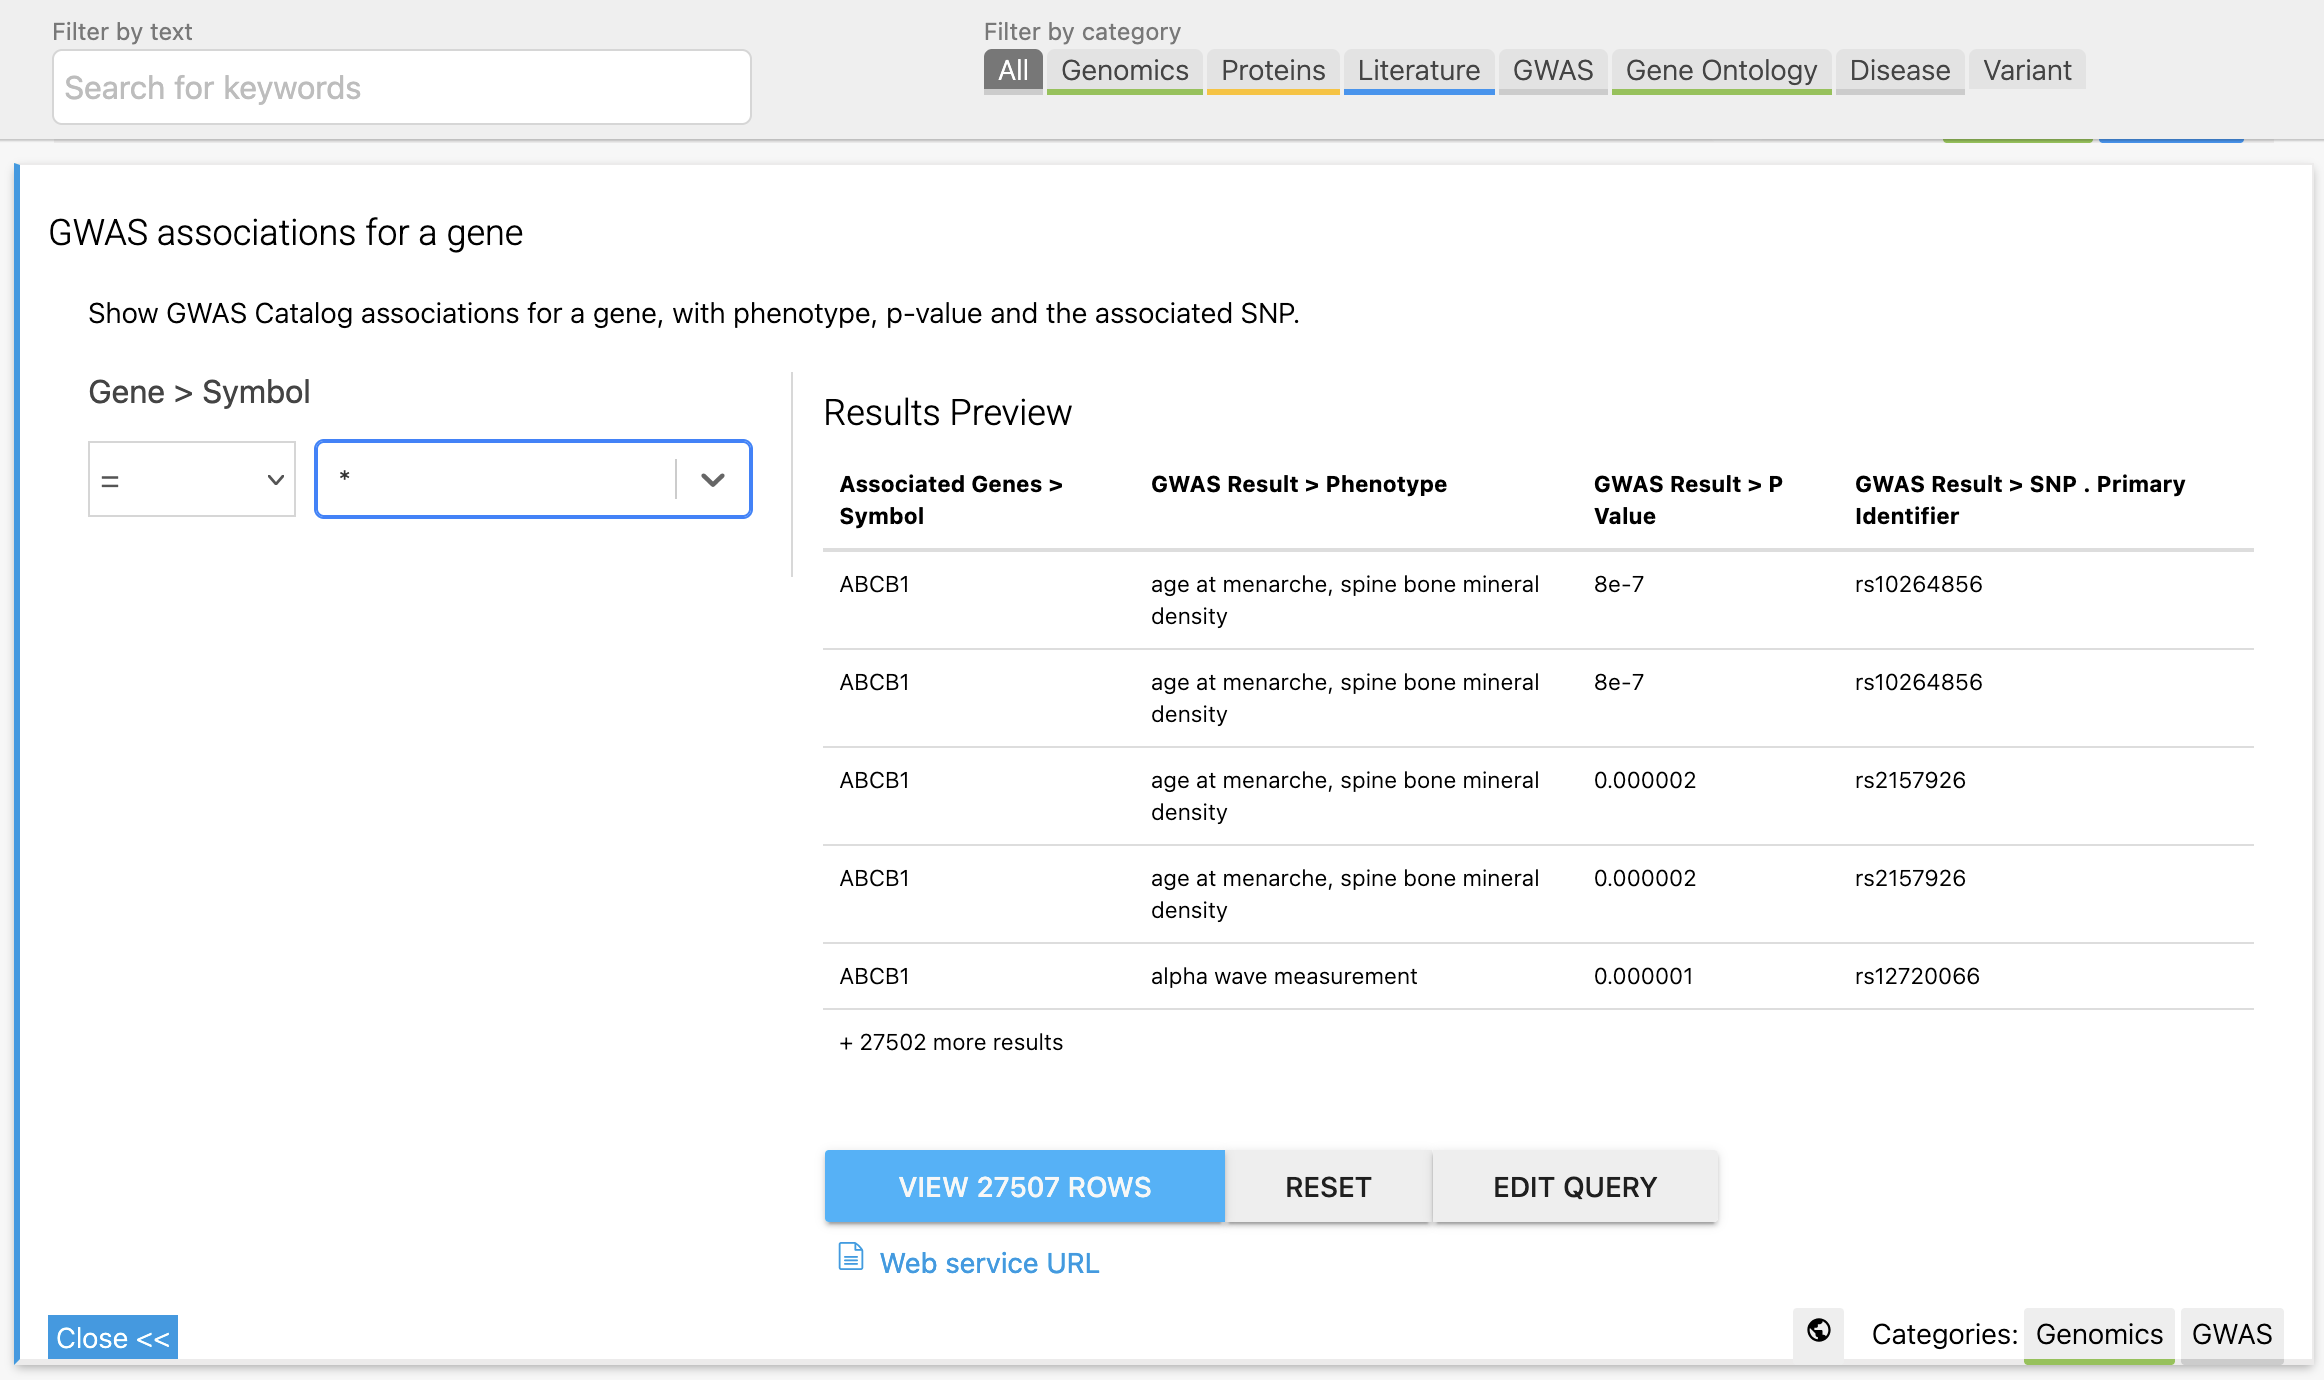
\includegraphics[width=\linewidth]{figure3-gwas-template.png}\\[0.8mm]
      {\fontsize{7.5}{9}\selectfont\color{muted}The running mine: a GWAS Catalog template
       added for the panel.\par}
    \end{column}
  \end{columns}

  \only<2>{%
  \begin{tikzpicture}[remember picture, overlay]
    \begin{scope}[shift={(current page.center)}, rotate=8]
      \fill[white, fill opacity=0.72] (-25mm,-25mm) rectangle (25mm,25mm);
      \draw[vermilion, line width=2.2mm, opacity=0.9] (-24mm,-24mm) rectangle (24mm,24mm);
      \draw[vermilion, line width=0.6mm, opacity=0.9] (-20mm,-20mm) rectangle (20mm,20mm);
      \node[vermilion, opacity=0.92] at (0, 8.6mm)
        {\sealfont\bfseries\fontsize{46}{46}\selectfont 共有};
      \node[vermilion, opacity=0.92] at (0,-9.4mm)
        {\sealfont\bfseries\fontsize{46}{46}\selectfont 財産};
    \end{scope}
    \node[fill=white, fill opacity=0.85, text opacity=1, rounded corners=1mm, inner sep=1.2mm]
      at ($(current page.center)+(0,-33mm)$)
      {\fontsize{10}{12}\selectfont\itshape kyōyū zaisan — shared asset};
  \end{tikzpicture}}
\end{frame}

% ------------------------------------------------- 4. What we learned, what's next
\begin{frame}[t]
  \vspace*{-3mm}
  \headline{The hard part is identity, not mapping}
  \vspace{2.5mm}
  {\fontsize{10.5}{13}\selectfont
  \begin{itemize}
    \setlength{\itemsep}{1.2mm}
    \item Which key does each object merge on?
    \item A gene needs its organism, as well as its identifier, to merge
    \item Some upstream keys are not unique: 255 Ensembl ids are claimed by
          more than one NCBI gene
  \end{itemize}\par}
  \vspace{2.5mm}
  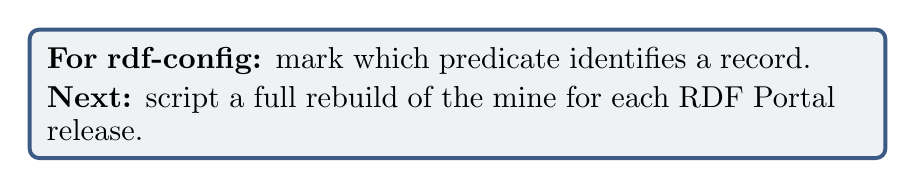
\begin{tikzpicture}
    \node[draw=shared, line width=0.5mm, fill=shared!8, rounded corners=1.2mm,
          inner sep=2.2mm, text width=0.86\textwidth, align=left]
      {\fontsize{10.5}{13}\selectfont\textbf{For rdf-config:} mark which predicate identifies a
       record.\\[0.8mm]
       \textbf{Next:} script a full rebuild of the mine for each RDF Portal release.};
  \end{tikzpicture}\par
  \vspace{2.2mm}
  {\fontsize{8.5}{10}\selectfont\color{muted}
   github.com/intermineorg/rdfc2im\qquad github.com/ryneches/rdfc2im-report\par}

  \begin{tikzpicture}[remember picture, overlay]
    \node[anchor=south, minimum width=\paperwidth, inner sep=1.2mm] (strip)
      at ($(current page.south)+(0,1mm)$)
      {
\includegraphics[height=6.5mm]{kuicr.png}\hspace{3.5mm}%
       
\includegraphics[height=6.5mm]{dbcls.pdf}\hspace{3.5mm}%
       \fbox{\parbox[c][5.5mm][c]{14mm}{\centering\fontsize{5}{6}\selectfont NIG logo\\(placeholder)}}\hspace{3.5mm}%
       
\includegraphics[height=5.5mm]{cambridge.pdf}\hspace{3.5mm}%
       
\includegraphics[height=6mm]{jst.pdf}\hspace{3.5mm}%
       
\includegraphics[height=6.5mm]{jsps.pdf}\hspace{3.5mm}%
       
\includegraphics[height=7.5mm]{bh26.png}};
    \node[anchor=south] at ($(strip.north)+(0,0.2mm)$)
      {\fontsize{6}{7}\selectfont\color{muted}
       Funding: JST DICP JPMJND2206 \textbullet\ JST GteX JPMJGX23B2 \textbullet\
       JSPS KAKENHI 23KK0122, 24K01889, 25K09119};
  \end{tikzpicture}
\end{frame}

\end{document}
